\chapter{内存管理}
\section{RISC-V页表硬件}

为了提高系统对物理内存的动态使用效率,隔离各应用的物理内存空间以保证应用间的安全性,我们对硬件层面的物理内存空间进行了一层抽象,建立了虚拟地址空间到物理内存空间的映射。从此,每个应用程序都享有独属于自己的,且足够庞大 (一般来说) 的存储空间,而不用与其他应用程序“抢占”资源。而将每个应用的逻辑地址空间分配到实际的物理内存空间这一任务,正是由操作系统来负责。

在分页内存管理中,操作系统通过“页表”来实现虚实内存映射机制,这是我们本章介绍的重点内容。同时,我们也可以使用页表来实现许多“有趣”的功能,例如将不同的地址空间映射至同一块物理内存空间,以实现共享内存;或是使用未映射的页面来保护内核和用户栈等等。

\subsection{虚拟地址与物理地址}

\subsubsection{地址的格式及关系}

如之前提到,实现虚拟地址到物理地址的映射,也就是页表的实现是我们本章的重点。不过在具体介绍页表之前,我们先来介绍我们所要维护的对象——虚拟地址与物理地址。

在Npucore中,虚拟地址空间和物理地址空间均采用页式管理,且每个页面的大小为 4KiB ($2^{12}$B)。如此一来,一个虚拟页面中的数据正好对应存储在一个物理页帧上,便于管理。根据页面大小的规定可知,每个页面需要使用12位字节地址来进行页内索引。根据页式管理的知识,我们将虚拟地址和物理地址均分成两部分:它们的低12位,即[11:0]被称为页内偏移 (Page Offset),它描述一个地址指向的字节在其所在页面中的相对位置。在SV39分页模式下,我们规定虚拟地址一共39位,则虚拟地址的高27位,即[38:12]为它的虚拟页号VPN (Virtual Page Number);我们规定物理地址一共56位,则物理地址的高44位,即[55:12]为它的物理页号PPN (Physical Page Number)。因此,地址的格式如图4-1所示:

\begin{figure}[h]
	\centering
	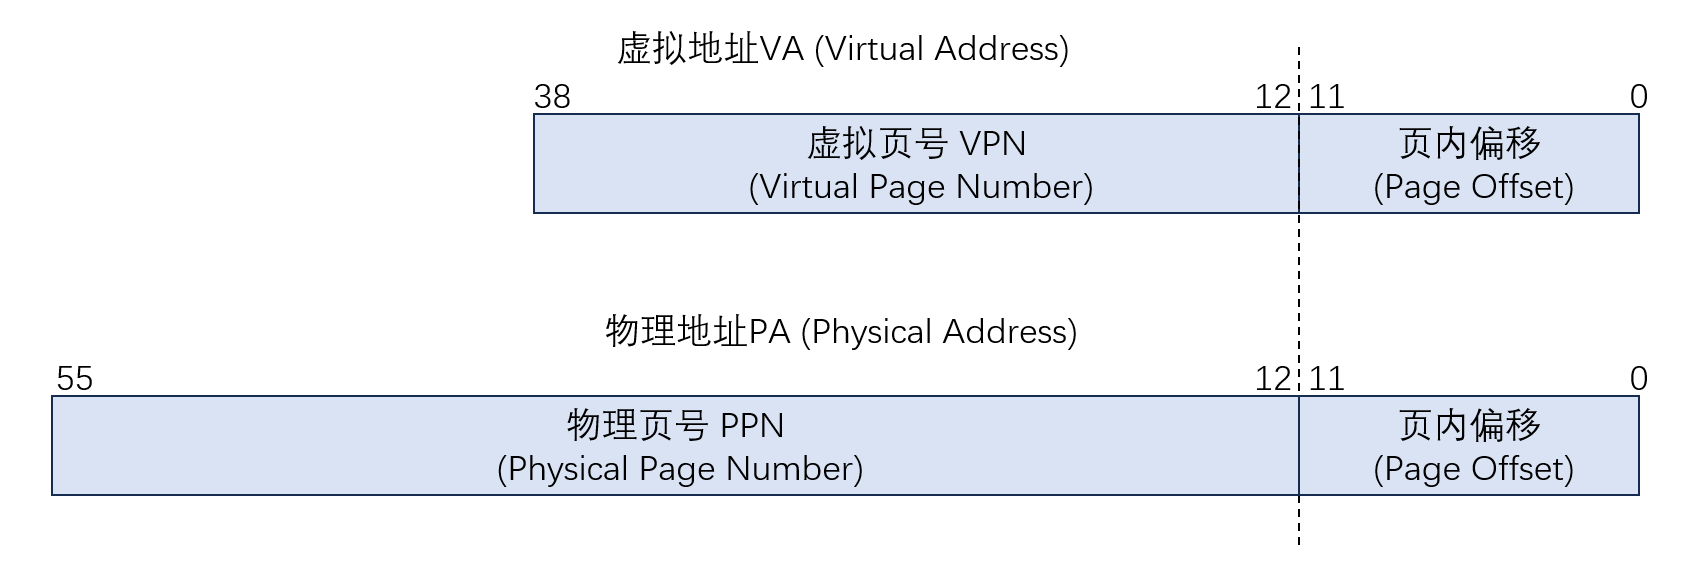
\includegraphics[width=.80\textwidth]{figures/04-01-虚拟地址与物理地址的格式.png}
	\caption{虚拟地址与物理地址的格式}
\end{figure}\FloatBarrier

回到我们的重点——地址转换。页式管理下,地址的转换是以页为单位进行的。也就是说,地址转换前后地址的页内偏移部分是不变的。因此,我们实际上要完成的操作是:从虚拟地址中取出27位虚拟页号,在页表中查询其对应的物理页号(若存在),最后将这27位虚拟页号映射得到的44位的物理页号与虚拟地址的12位页内偏移按序拼接到一起,就得到了56位的物理地址,完成了地址转换的过程。

\subsubsection{地址的数据结构抽象}

物理地址共有56位,这是由RISC-V的硬件设计人员决定的。但在64位的架构上,虚拟地址长度确实应该和位宽一致,为64位。不过在SV39分页模式下,虚拟地址只有低39位是有实际意义的。SV39分页模式规定64位虚拟地址的高25位必须和第38位相同,否则内存管理单元(MMU)会直接认定它是一个不合法的虚拟地址。通过这个检查之后,MMU再取出低39位尝试将其转化为一个56位的物理地址。同样,为了易于数据结构的实现,我们也将物理地址以64位进行封装。具体的实现如下:

\begin{lstlisting}[language={Rust}, label={code:address},
		caption={os/src/mm/address.rs}]
// Definitions
#[repr(C)]
#[derive(Copy, Clone, Ord, PartialOrd, Eq, PartialEq)]
pub struct PhysAddr(pub usize);

#[repr(C)]
#[derive(Copy, Clone, Ord, PartialOrd, Eq, PartialEq)]
pub struct VirtAddr(pub usize);
	
#[repr(C)]
#[derive(Copy, Clone, Ord, PartialOrd, Eq, PartialEq)]
pub struct PhysPageNum(pub usize);

#[repr(C)]
#[derive(Copy, Clone, Ord, PartialOrd, Eq, PartialEq)]
pub struct VirtPageNum(pub usize);
\end{lstlisting}

上面分别给出了物理地址PA、虚拟地址VA、物理页号PPN、虚拟页号VPN的类型声明,它们都是元组式结构体,可以看成usize的一种简单包装。我们刻意将它们各自抽象出不同的类型而不是都使用与RISC-V 64硬件直接对应的usize基本类型,是为了在Rust编译器的帮助下,通过多种安全且方便的类型转换来构建页表。

实现这些地址信息类型与usize类型之间的相互转换,需要使用From<T> trait (同时实现了Into<T> trait)。这里我们以PPN为例,介绍其与usize类型的转换(其余三种地址信息类型PA、VA、VPN的实现均一致,仅有类型声明的差异)。对usize类型实现以下trait,使我们可以使用usize类型数据生成一个PhysPageNum类型的数据:

\begin{lstlisting}[language={Rust}, label={code:address},
	caption={os/src/mm/address.rs}]
impl From<usize> for PhysPageNum {
	fn from(v: usize) -> Self {
		Self(v)
	}
}
\end{lstlisting}

反过来,同样对PhysPageNum类型实现该trait,使我们可以使用PhysPageNum类型数据生成一个usize类型的数据:

\begin{lstlisting}[language={Rust}, label={code:address},
	caption={os/src/mm/address.rs}]
impl From<PhysPageNum> for usize {
	fn from(v: PhysPageNum) -> Self {
		v.0
	}
}
\end{lstlisting}

至此,我们实现了地址信息类型与usize类型的相互转换。注意到,从地址信息变量(以PPN为例)得到它的usize类型的更简便方法是直接ppn.0。

同时,我们也支持地址类型与页号类型的相互转换。需要注意的是,从页号到地址的转换只需左移12位即可;而地址转换至页号则必须保证它与页面大小对齐(即页内偏移为0),若不对齐,则需要先进行取整。接下来以物理地址与物理页号的转换为例:

首先介绍地址的取整:

\begin{lstlisting}[language={Rust}, label={code:address},
	caption={os/src/mm/address.rs}]
impl PhysAddr {
	pub fn floor(&self) -> PhysPageNum {
		PhysPageNum(self.0 / PAGE_SIZE)
	}
	pub fn ceil(&self) -> PhysPageNum {
		PhysPageNum((self.0 + PAGE_SIZE - 1) / PAGE_SIZE)
	}
}
\end{lstlisting}

floor为下取整方法,而ceil为上取整方法。其中,PAGE\_SIZE为4096,表示每个页面的大小。

接下来介绍地址与页号的转换,我们同样是实现From<T> trait:

\begin{lstlisting}[language={Rust}, label={code:address},
	caption={os/src/mm/address.rs}]
impl PhysAddr {
	pub fn page_offset(&self) -> usize { self.0 & (PAGE_SIZE - 1) }
}

impl From<PhysAddr> for PhysPageNum {
	fn from(v: PhysAddr) -> Self {
		assert_eq!(v.page_offset(), 0);
		v.floor()
	}
}

impl From<PhysPageNum> for PhysAddr {
	fn from(v: PhysPageNum) -> Self { Self(v.0 << PAGE_SIZE_BITS) }
}
\end{lstlisting}

其中,PAGE\_SIZE\_BITS为12,表示页内偏移的位宽。

至此,我们对地址信息类型的实现已经有了基本的掌握。

\subsection{页表项}

\subsubsection{页表项格式及含义}

在上面的内容中其实我们已经认识到,虚实地址转换的流程核心就是:使用虚拟页号作为索引在页表中查询到对应的物理页号。若把页表比作一个货架,则虚拟页号就是商品的编号,我们通过这个编号寻找到对应的商品,而这个商品就存储着我们需要的物理地址信息。“这个商品”指的就是页表项。

SV39分页模式下,页表项是一个8字节的比特序列,其结构如图4-2所示:

\begin{figure}[h]
	\centering
	\includegraphics[width=.80\textwidth]{figures/04-02-页表项的格式.png}
	\caption{页表项的格式}
\end{figure}\FloatBarrier

可见,[63:54]这10位是保留位,被忽略;[53:10]这44位是物理页号;而最低的10位[9:0]则是标志位。标志位实际上控制了应用对其地址空间中每个虚拟页面的访问权限,他们的具体含义如下:

\begin{itemize}
	\item [$\bullet$]
	V(Valid):有效位。仅当V为1时,该页表项合法;
	\item [$\bullet$]
	R(Read)/W(Write)/X(eXecute):分别表示索引到这个页表项的对应虚拟页面是否允许读/写/执行;
	\item [$\bullet$]
	U(User):表示索引到这个页表项的对应虚拟页面是否在CPU处于U特权级的情况下允许访问;
	\item [$\bullet$]
	G(Global):全局标志。为1时表明该页面为全局页面;
	\item [$\bullet$]
	A(Accessed):处理器使用此位来记录自页表项上的这一位被清零后,其对应虚拟页面是否被访问过;
	\item [$\bullet$]
	D(Dirty):处理器使用此位来记录自页表项上的这一位被清零后,其对应虚拟页面是否被修改过;
	\item [$\bullet$]
	RSW(Reserved for Supervisor softWare):保留位。该部分被处理器忽略,软件可以使用。	
\end{itemize}

总之,页表项不仅存储了物理地址信息,还存储了一组标志位用于对虚拟页面的权限控制。

\subsubsection{页表项的数据结构抽象}

首先我们对标志位使用bitflags!宏进行包装:

\begin{lstlisting}[language={Rust}, label={code:pte},
	caption={os/src/mm/page\_table.rs}]
use bitflags::*;
bitflags! {
	pub struct PTEFlags: u8 {
		const V = 1 << 0;
		const R = 1 << 1;
		const W = 1 << 2;
		const X = 1 << 3;
		const U = 1 << 4;
		const G = 1 << 5;
		const A = 1 << 6;
		const D = 1 << 7;
	}
}
\end{lstlisting}

可见,我们将一个u8类型封装成了一个标志位的集合类型PTEFlags,使其支持一些常见的集合运算,且使用时易于理解。

接下来我们实现页表项PageTableEntry:

\begin{lstlisting}[language={Rust}, label={code:pte},
	caption={os/src/mm/page\_table.rs}]
#[derive(Copy, Clone)]
#[repr(C)]
pub struct PageTableEntry {
	pub bits: usize,
}

impl PageTableEntry {
	pub fn new(ppn: PhysPageNum, flags: PTEFlags) -> Self {
		PageTableEntry {
			bits: ppn.0 << 10 | flags.bits as usize,
		}
	}
}
\end{lstlisting}

可见,PageTableEntry类型实际上也是对usize类型的一层简单包装。new方法使得我们可以从一个PhysPageNum类型的物理页号和一个PTEFlags类型的页表项标志位生成一个页表项实例。当然,我们也提供了一些简单的方法,用于取出或直接使用页表项中的信息,例如:

\begin{lstlisting}[language={Rust}, label={code:pte},
	caption={os/src/mm/page\_table.rs}]
impl PageTableEntry {
	pub fn ppn(&self) -> PhysPageNum {
		(self.bits >> 10 & ((1usize << 44) - 1)).into()
	}
	pub fn flags(&self) -> PTEFlags {
		PTEFlags::from_bits(self.bits as u8).unwrap()
	}
	pub fn is_valid(&self) -> bool {
		(self.flags() & PTEFlags::V) != PTEFlags::empty()
	}
}
\end{lstlisting}

前两个方法与new方法相对,可以从一个页表项实例中取出物理页号或标志位信息。最后一个方法可以快速判断当前页表项是否合法。当然,还有许多相似的辅助函数在此没有介绍。

至此,我们对页表项的结构以及使用也有了一个基本的了解,下面我们终于可以介绍页表了。

\subsection{页表}

\subsubsection{SV39三级页表结构}

在上一节中,我们将页表比作了一个货架,而货架上装的是页表项PTE这一商品。事实上,页表的确可以看作是一组页表项的集合,且这种集合的组织形式是最简单的线性表,当然这是对于一个页表而言。实际上,如果我们只维护一张页表来将高达512GiB的虚拟地址空间进行映射,页表本身就会变得相当庞大,远超出我们的实际物理内存。因此,SV39模式使用了三级页表结构,将原本一张巨大的页表拆分成许许多多的小页表,再将这些页表通过树状结构组织起来,以此提高信息的利用率,从而节省空间。注意:这里的树状结构指的是页表与页表之间的关系,而一个页表本身仍为一份线性表,里面存储了若干页表项。接下来我们将详细介绍这一结构,介绍完结构后,我们会阐明这么做的原因。

首先,在SV39模式下,一张页表正好占据一张物理页帧。由于一个页表项是8字节,因此每个页表需要保存4KiB/8B=512个页表项,这些页表项线性排列在页表内,如图4-3:

\begin{figure}[h]
	\centering
	\includegraphics[width=.80\textwidth]{figures/04-03-单个页表的结构.png}
	\caption{单个页表的结构}
\end{figure}\FloatBarrier

上图逐层对页表的结构进行了刻画。请留意这张图,我们在对页表进行数据结构抽象时还会用到。接下来我们来介绍页表间的树状结构:

我们多次强调,树状结构指的是页表间的结构,也就是说,我们要将一个页表视为一个节点,并将这些节点以树状形式相连。换句话说,我们要从一个页表出发,对应到若干个子页表,这要怎么做到呢?

回想两个已知的事实:\ding{192}一张页表恰好位于一个物理页帧上,而一个物理页帧由一个物理页号标识。换句话说,一张页表由其所在物理页帧的物理页号唯一标识。\ding{193}页表中存储的是若干条PTE,而每个PTE存储着一个物理页号以及若干标志位。

至此,方法已水到渠成:我们可以使用PTE来记录页表的位置,从而实现页表至页表间的关联。在上一节中我们说,PTE存储的是虚拟页号所对应的物理页号。而现在我们要将一部分PTE进行改造,使其存储的物理页号信息不再与虚拟页号直接对应,而是与页表所在的物理页帧对应。注意这种改造并非改变PTE的结构,仅是改变PTE的逻辑含义,改造方法将会在本小节最后给出。

因此,现在我们具有两种不同的PTE:一种PTE存储的是我们最终需要的、虚拟页号所直接对应的物理页号,这种PTE存储于位于叶子节点的页表中;第二种PTE是经过我们改造的,存储指向一个页表的物理页号,这种PTE存储于非叶子节点的页表中。至此,我们已经构建起了页表与页表间的联系,将他们按树状结构组织,如图4-4:

\begin{figure}[h]
	\centering
	\includegraphics[width=.80\textwidth]{figures/04-04-三级页表结构.png}
	\caption{三级页表结构}
\end{figure}\FloatBarrier

如图,SV39中页表以三级的树结构组织在一起。树的根节点被称为一级页表节点,一级页表节点存储着二级页表节点的位置信息;同样二级页表节点存储着三级页表节点的位置信息;而三级页表节点是树的叶子节点,存储着最终虚拟页号所对应的物理页号。

下面我们来谈谈这种页表组织形式的好处:

前面我们提到,之所以不维护一个记录全部映射关系的页表,是因为它保存了所有虚拟页号对应的页表项,远超我们内存空间的上限。实际上,高达512GiB的虚拟地址空间真正会被使用到的只是其中极小的一部分,也就是说这种页表的绝大部分空间都是被浪费掉的。因此,我们需要“按需分配”,使得页表中存储的是真正有意义的、会被使用到的页表项。

一开始每个应用的地址空间都是空的,此时的页表也应为空。而当内核决定好了一个应用的各逻辑段存放位置后,MMU就从零开始,以虚拟页面为单位来让该应用的地址空间的某些部分与实际物理内存空间相对应,反映在本应用的页表上就是一对对映射顺次被插入进来。

因此,我们需要一个动态的、支持页表所占据的内存大小随映射数量增加而增加的页表结构,最终我们选择了树状结构。实际操作中,每个应用最初只有一个一级页表,仅占据一个物理页帧大小。而当映射开始插入后,页表从根节点开始“发芽抽枝”,逐步增加二级页表与三级页表,增加的每个页表也仅占一个物理页帧空间。就这样,这种三级页表结构以低粒度的形式保证了页表大小的动态变化,解决了单一页表占据空间过大的问题。

最后,我们解释如何赋予PTE两种不同的含义:存储的PPN指向一个页表或是指向我们最终所需的物理页号。其实这十分容易,我们正是通过操作PTE的符号位来实现这一区分,在此我们直接给出SV39中PTE符号位R/W/X组合的含义,通过这三个符号的组合我们可以了解该PTE的具体属性:

\begin{table}[h]
\begin{center}
表4-1 PTE的R/W/X符号位编码 \\
\begin{tabular}{|c|cc|c}
	\hline
	X & \multicolumn{1}{c|}{W} & R & \multicolumn{1}{c|}{含义} \\
	\hline
	0 & \multicolumn{1}{c|}{0} & 0 & \multicolumn{1}{l|}{本PTE存储的PPN指向下一级页表} \\
	0 & \multicolumn{1}{c|}{0} & 1 & \multicolumn{1}{l|}{指向本PTE的虚拟页面为只读页} \\
	0 & \multicolumn{1}{c|}{1} & 0 & \multicolumn{1}{l|}{保留,暂无用} \\
	0 & \multicolumn{1}{c|}{1} & 1 & \multicolumn{1}{l|}{指向本PTE的虚拟页面为可读写页} \\
	1 & \multicolumn{1}{c|}{0} & 0 & \multicolumn{1}{l|}{指向本PTE的虚拟页面为只可执行页} \\
	1 & \multicolumn{1}{c|}{0} & 1 & \multicolumn{1}{l|}{指向本PTE的虚拟页面为可读可执行页} \\
	1 & \multicolumn{1}{c|}{1} & 0 & \multicolumn{1}{l|}{保留,暂无用} \\
	1 & \multicolumn{1}{c|}{1} & 1 & \multicolumn{1}{l|}{指向本PTE的虚拟页面为可读写可执行页} \\
	\hline
\end{tabular}
\end{center}
\end{table}\FloatBarrier

注意,上表成立的前提是PTE的V (Valid) 标志位为1。当V为0的时候,代表当前PTE是无效的。

\subsubsection{页表的数据结构抽象}

我们在之前已经提到,SV39模式下,每个页表恰好占据一个物理页帧的空间,因此每个页表可以用一个物理页号来标识。

\begin{lstlisting}[language={Rust}, label={code:pagetable},
	caption={os/src/mm/page\_table.rs}]
pub struct PageTable {
	root_ppn: PhysPageNum,
	frames: Vec<FrameTracker>,
}

impl PageTable {
	pub fn new() -> Self {
		let frame = frame_alloc().unwrap();
		PageTable {
			root_ppn: frame.ppn,
			frames: vec![frame],
		}
	}
}
\end{lstlisting}

可见,PageTable类型保存了其所在的物理页帧的页号作为其唯一标识。此外还有一个frames字段,该字段主要用于实现页表映射的物理页帧的生命周期与页表同步,其具体功能实现我们将在物理页帧管理模块再继续介绍。

由于页表使用物理页号进行标识,因此我们已经可以方便地使用PTE来寻找对应的页表位置,即非叶子节点的页表中的PTE存储的PPN,即为一个页表的root\_ppn。那么,我们怎么通过页表来取得其存储的PTE呢?需要用到以下方法:

\begin{lstlisting}[language={Rust}, label={code:address},
	caption={os/src/mm/page\_table.rs}]
impl PhysPageNum {
	pub fn get_pte_array(&self) -> &'static mut [PageTableEntry] {
		let pa: PhysAddr = self.clone().into();
		unsafe {
			core::slice::from_raw_parts_mut(pa.0 as *mut PageTableEntry, 512)
		}
	}
}
\end{lstlisting}

该方法构造可变引用来直接访问一个物理页号对应的物理页帧,然后正如图4-3的第一个箭头那样,将页表所在的物理页帧切分成512份,每一份正是对应一项PTE,最终该方法返回一个页表项类型的定长数组(长度为512)的可变引用,代表了多级页表中的一个节点。至此,我们也实现了从一个页表获取其页表项的方法。万事俱备,现在我们可以介绍虚实地址的映射过程了。

\subsection{虚实地址的映射过程}

\subsubsection{satp寄存器} 

首先我们介绍一个寄存器——satp寄存器。

该寄存器存储了与分页模式有关的信息。默认情况下,内存管理单元MMU未被使能(启用),此时无论CPU位于哪个特权级,访存的地址都会作为一个物理地址交给对应的内存控制单元来直接访问。通过修改S特权级的satp寄存器可以启用分页模式,在这之后S和U特权级的访存地址会被视为一个虚拟地址,它需要经过MMU的地址转换变为一个物理地址,再通过它来访问物理内存。

下面给出RISC-V 64架构下satp的字段分布,如图4-5:

\begin{figure}[h]
	\centering
	\includegraphics[width=.80\textwidth]{figures/04-05-satp寄存器的字段结构.png}
	\caption{satp寄存器的字段结构}
\end{figure}\FloatBarrier

各字段含义如下:

\begin{itemize}
	\item [$\bullet$]
	MODE:控制CPU使用何种分页模式。当MODE设置为0的时候,代表所有访存都被视为物理地址;而设置为8的时候,SV39分页机制被启用;
	\item [$\bullet$]
	ASID:表示地址空间标识符,与进程管理有关,此处先不介绍;
	\item [$\bullet$]
	PPN:该PPN是当前地址空间的根页表所在的物理页号。这样,给定一个虚拟页号,CPU就可以从三级页表的根页表开始一步步的将其映射到一个物理页号,也就是说,页表的使用入口存储于此。
\end{itemize}

\subsubsection{三级页表的使用流程}

我们知道,SV39模式中的虚拟页号为27位,而这其实是大有深意的。对于一个虚拟地址来说,将其[38:12]这27位的虚拟页号分为三个等长的部分,每个部分9位,即[38:30]为$VPN_{1}$,[29:21]为$VPN_{2}$,[20:12]为$VPN_{3}$。这样,每个$VPN_{i}$均能标识$2^{9}$=512个单位。看到这里读者是否想起些什么?没错,我们每个页表所存储的PTE数组长度正好是512,事实上,每个虚拟页号的三个分段也正是对应着其在三级页表中的索引。所以,一个虚拟地址通过页表转化为物理地址的流程如下:

\begin{itemize}
	\item [\ding{192}]
	通过satp中的PPN字段找到一级页表(根页表);
	\item [\ding{193}]
	在一级页表中,将$VPN_{1}$作为索引查询到对应的PTE,通过该PTE中的PPN字段找到二级页表;
	\item [\ding{194}]
	在二级页表中,将$VPN_{2}$作为索引查询到对应的PTE,通过该PTE中的PPN字段找到三级页表;
	\item [\ding{195}]
	在三级页表中,将$VPN_{3}$作为索引查询到对应的PTE,通过该PTE中的PPN字段找到本虚拟页号所对应的物理页号;
	\item [\ding{196}]
	将得到的物理页号与本虚拟地址的低12位偏移量拼凑在一起,即获得了最终对应的物理地址。
\end{itemize}

该流程的图示如图4-6:

\begin{figure}[h]
	\centering
	\includegraphics[width=.80\textwidth]{figures/04-06-虚实地址转换流程.png}
	\caption{虚实地址转换流程}
\end{figure}\FloatBarrier

\subsubsection{Npucore中的方法实现}

在Npucore中,我们使用PageTable类型的translate\_va方法来实现虚拟地址到物理地址的转换:

\begin{lstlisting}[language={Rust}, label={code:pte},
	caption={os/src/mm/page\_table.rs}]
pub fn translate_va(&self, va: VirtAddr) -> Option<PhysAddr> {
	self.find_pte(va.clone().floor()).map(|pte| {
		let aligned_pa: PhysAddr = pte.ppn().into();
		let offset = va.page_offset();
		let aligned_pa_usize: usize = aligned_pa.into();
		(aligned_pa_usize + offset).into()
	})
}
\end{lstlisting}

该方法的核心实际上是调用了find\_pte方法,完成从虚拟页号查询到叶子节点的对应PTE的过程。第3行是从最终查询到的PTE获取物理地址的PPN段,而4、5、6行实际上是完成了一个物理地址的拼接过程。map是一个泛型闭包,将最后拼接而成的usize类型转化为PhysAddr类型。我们接下来看find\_pte方法的实现:

\begin{lstlisting}[language={Rust}, label={code:pte},
	caption={os/src/mm/page\_table.rs}]
fn find_pte(&self, vpn: VirtPageNum) -> Option<&PageTableEntry> {
	let idxs = vpn.indexes();
	let mut ppn = self.root_ppn;
	let mut result: Option<&PageTableEntry> = None;
	for i in 0..3 {
		let pte = &ppn.get_pte_array()[idxs[i]];
		if !pte.is_valid() {
			return None;
		}
		if i == 2 {
			result = Some(pte);
			break;
		}
		ppn = pte.ppn();
	}
	result
}
\end{lstlisting}

由于find\_pte是一个页表类型下的方法,其在调用时对应一个页表实例。而由于每个地址空间总是保存着其根页表的位置信息(satp寄存器),因此该方法的调用者总是根页表,相当于我们已经实现了取得根页表的第一步。因此本方法实际就是实现对三级页表树的查询。

第2行,调用indexes方法:

\begin{lstlisting}[language={Rust}, label={code:pte},
	caption={os/src/mm/address.rs}]
impl VirtPageNum {
	pub fn indexes(&self) -> [usize; 3] {
		let mut vpn = self.0;
		let mut idx = [0usize; 3];
		for i in (0..3).rev() {
			idx[i] = vpn & 511;
			vpn >>= 9;
		}
		idx
	}
}
\end{lstlisting}

该方法将VPN切分为三份,返回一个长度为3的usize类型数组,即$VPN_{1}$,$VPN_{2}$,$VPN_{3}$的信息。

第3行,我们获取当前页表的root\_ppn,是为了后续调用get\_pte\_array方法来取得页表中存储的PTE。

从第5行开始,我们通过3次的for循环来进行三级页表的查询,每次循环均通过对应的VPN片段在页表中获取PTE,然后判断该PTE的有效性以及其所在的页表是否位于叶子节点:若非叶子节点,则取出该PTE的PPN定位下一级页表;若为叶子节点,则直接返回当前PTE。

至此,我们按照图4-6完成了虚实地址转换的实现。

\subsection{TLB}

我们知道,物理内存的访问速度要比CPU的运行速度慢很多。如果我们按照上面介绍的三级页表机制循规蹈矩地查询,将一个虚拟地址转化为物理地址需要访问3次物理内存,得到物理地址后还需要再访问一次物理内存,才能完成全部访存操作,这无疑很大程度上降低了系统执行效率。

我们在计算机组成原理课程中学习过Cache的设计理念,即利用地址访问过程的时间局部性和空间局部性特点,将内存上的部分数据拉取至缓存中,加快CPU的访问速度。实际上,我们对于页表也是这么做的,我们使用一个速度比较快的缓存TLB (Translation Lookaside Buffer),也称为快表,将页表中最近使用的PTE缓存下来。

从本质上来讲,TLB就是页表的Cache。但是TLB不同于一般的Cache,它只有时间相关性,也就是说,现在访问的页,很有可能在以后继续被访问。至于空间相关性,TLB并没有明显的规律,因为在一个页内有很多情况,都可能使程序跳转到其他不相邻的页中取指令或数据,也就是说,虽然当前在访问一个页,但未必会访问它相邻的页。正因为如此,Cache设计中很多的优化方法,例如预取 (prefetching),是没有办法应用于TLB中的。

对于TLB的写入、缺失处理、控制等相关知识可在计算机组成原理课程中进一步学习。
